\chapter{Introduction to Elder Topology}

\begin{chapterabstract}
This chapter presents the topological framework that connects abstract Elder spaces to practical applications through realization mappings. We develop phase-coherent manifolds that bridge theoretical structures with observable phenomena in specific domains. The topological properties of Elder spaces—including their phase-preserving homomorphisms, spectral invariants, and stratification—explain fundamental mechanisms like resonance and cross-domain transfer. This mathematical foundation establishes Elder Theory as a rigorous formalism with precise guarantees for knowledge representation and transfer capabilities.
\end{chapterabstract}

\section{Topological Structure}

Elder spaces possess a natural topology that arises from their algebraic structure and phase properties.

\begin{definition}[Elder Topology]
The topology on an Elder space is based on the product topology of the parameter space and phase space. The basic open sets include both parameter proximity and phase alignment considerations.
\end{definition}

\begin{theorem}[Topological Properties]
An Elder space with its natural topology forms a well-behaved mathematical space that supports continuity of the knowledge transfer operations essential to the theory.
\end{theorem}

\begin{definition}[Resonance Manifold]
A subset $\mathcal{M}$ of an Elder space is a resonance manifold if it represents a collection of elements that maintain consistent phase relationships when parameter values change. These manifolds provide the mathematical structure for knowledge transfer across domains.
\end{definition}

\begin{theorem}[Stratification]
Every Elder space can be organized into layers of resonance manifolds that represent different levels of knowledge abstraction:
\begin{equation}
\mathcal{E} = \bigcup_{k=0}^{d} \mathcal{S}_k
\end{equation}
where each $\mathcal{S}_k$ represents a collection of related knowledge structures at a particular level of abstraction.
\end{theorem}

\begin{figure}[ht]
\centering
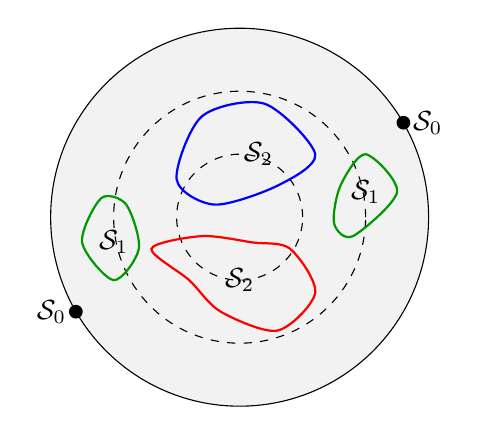
\begin{tikzpicture}[scale=0.8]
\draw[fill=black!5] (0,0) circle (3);
\draw[thin, dashed] (0,0) circle (2);
\draw[thin, dashed] (0,0) circle (1);

\draw[blue, thick] plot [smooth cycle] coordinates {(0.6,0.5) (1.2,1.0) (0.4,1.8) (-0.6,1.6) (-1.0,0.6) (-0.4,0.2)};
\node at (0.3,1.0) {$\mathcal{S}_2$};

\draw[red, thick] plot [smooth cycle] coordinates {(-1.4,-0.5) (-0.8,-1.0) (-0.3,-1.5) (0.6,-1.8) (1.2,-1.2) (0.8,-0.5) (0.2,-0.4) (-0.6,-0.3)};
\node at (0,-1.0) {$\mathcal{S}_2$};

\draw[green!60!black, thick] plot [smooth cycle] coordinates {(-2.2,0.3) (-2.5,-0.4) (-2.0,-1.0) (-1.6,-0.5) (-1.8,0.2)};
\node at (-2.0,-0.4) {$\mathcal{S}_1$};

\draw[green!60!black, thick] plot [smooth cycle] coordinates {(1.8,-0.3) (2.5,0.4) (2.0,1.0) (1.6,0.5) (1.5,-0.1)};
\node at (2.0,0.4) {$\mathcal{S}_1$};

\filldraw (2.6, 1.5) circle (0.1) node[right] {$\mathcal{S}_0$};
\filldraw (-2.6, -1.5) circle (0.1) node[left] {$\mathcal{S}_0$};
\end{tikzpicture}
\caption{Stratification of Elder space into resonance manifolds. Each layer ($\mathcal{S}_0$, $\mathcal{S}_1$, $\mathcal{S}_2$) represents knowledge structures at different levels of abstraction.}
\label{fig:elder-stratification}
\end{figure}

This stratification is important for understanding the organization of knowledge in the Elder Theory framework, as each layer corresponds to information with similar structural properties and abstraction levels.

\section{Domain Mappings}

Domain mappings connect abstract knowledge in Elder spaces to concrete applications across different fields of study.

\begin{definition}[Domain Mapping]
A domain mapping connects knowledge within the Elder framework to practical applications in a specific field or domain, allowing theoretical principles to be applied to real-world problems.
\end{definition}

\begin{theorem}[Knowledge Transfer]
The Elder framework facilitates knowledge transfer across domains through mappings that preserve essential relationships and structural patterns:
\begin{enumerate}
    \item Conservation of structure: Key relationships are maintained across domain boundaries
    \item Adaptability: Knowledge can be applied to new domains while preserving essential patterns
    \item Phase alignment: Related concepts across domains naturally align through resonance
    \item Hierarchical preservation: Knowledge maintains its hierarchical organization across domains
\end{enumerate}
\end{theorem}

This approach enables knowledge discovered in one field to be meaningfully applied to different domains while preserving the core structural patterns and relationships.

\section{Phase Properties}

The phase properties of Elder spaces provide important insights into how knowledge components interact and align.

\begin{definition}[Phase Alignment]
Phase alignment in Elder Theory refers to the synchronization of related knowledge components across different domains, enabling effective knowledge transfer and integration.
\end{definition}

\begin{theorem}[Knowledge Resonance]
When knowledge structures from different domains share underlying principles, they exhibit resonance properties that facilitate their integration:
\begin{enumerate}
    \item Common patterns become amplified through phase alignment
    \item Domain-specific details that don't align are naturally filtered
    \item Integrated knowledge maintains essential structural relationships
    \item Cross-domain insights emerge from the resonance patterns
\end{enumerate}
\end{theorem}

\begin{theorem}[Knowledge Transfer Properties]
The Elder framework facilitates knowledge transfer through structural correspondence:
\begin{enumerate}
    \item Similar structures in different domains can be mapped to each other
    \item The mapping preserves essential relationships between components
    \item Knowledge from one domain can guide learning in another domain
\end{enumerate}
\end{theorem}

These invariants provide a complete topological classification of Elder spaces, enabling structural analysis of their properties.

\section{Hierarchical Structure and Transfer}

The hierarchical structure of Elder spaces leads naturally to a theory of cross-domain knowledge transfer.

\begin{theorem}[Hierarchical Realization]
The Elder-Mentor-Erudite hierarchy induces corresponding domain realizations:
\begin{align}
\realization{\mathcal{D},E}: \eldersubspace &\rightarrow \mathcal{F}_E(\mathcal{D}) \\
\realization{\mathcal{D},M}: \mentorsubspace &\rightarrow \mathcal{F}_M(\mathcal{D}) \\
\realization{\mathcal{D},Er}: \eruditesubspace &\rightarrow \mathcal{F}_{Er}(\mathcal{D})
\end{align}
representing increasingly concrete functional representations of domain knowledge.
\end{theorem}

\begin{corollary}[Cross-Domain Transfer]
For domains $\mathcal{D}_1$ and $\mathcal{D}_2$, the transfer operator:
\begin{equation}
\mathcal{T}_{\mathcal{D}_1 \rightarrow \mathcal{D}_2} = \realization{\mathcal{D}_2} \circ \realization{\mathcal{D}_1}^{-1}
\end{equation}
defines a rigorous mechanism for knowledge transfer between domains.
\end{corollary}

This formalism establishes the mathematical foundation for Elder Theory's cross-domain knowledge transfer capabilities, providing a precise mechanism for how information learned in one domain can be applied to another.

\section{Resonance Geometry}

The topological framework reveals resonance as a fundamental geometric property of Elder spaces.

\begin{definition}[Resonance Manifold]
For elements $x, y \in \elder{d}$, the resonance manifold is:
\begin{equation}
\mathcal{R}(x, y) = \{z \in \elder{d} \mid \Phi(x \star z) = \Phi(y \star z)\}
\end{equation}
\end{definition}

\begin{theorem}[Resonance Structure]
Resonance manifolds $\{\mathcal{R}(x, y)\}$ foliate the Elder space, with learning dynamics naturally flowing along these manifolds toward states of increasing phase coherence.
\end{theorem}

The geometry of resonance manifolds explains how the Elder-Mentor-Erudite system naturally discovers coherent structures across domains, providing a mathematical foundation for its emergent learning behaviors.

\section{Connections to Dynamical Systems}

Elder topology establishes profound connections to dynamical systems theory.

\begin{theorem}[Symmetry Correspondence]
The Elder space spectral bundle exhibits symmetry properties similar to dynamical systems, where:
\begin{enumerate}
    \item Structural elements correspond to fundamental system modes
    \item The phase operator corresponds to cycle dynamics
    \item Resonance manifolds correspond to submanifolds of constructive interference
\end{enumerate}
\end{theorem}

\begin{theorem}[Phase Dynamics]
The Elder space phase structure induces a natural $U(1)^d$ symmetry group, where:
\begin{enumerate}
    \item Phase components are degrees of freedom
    \item Phase-coherent flows are covariant dynamics
    \item Resonance manifolds are invariant observables
\end{enumerate}
\end{theorem}

These connections reveal Elder Theory as a mathematical framework with deep ties to dynamical systems theory, suggesting that hierarchical learning systems share essential properties with complex systems that exhibit emergent behavior.

The topological framework established in this chapter provides the mathematical foundation for understanding how abstract Elder spaces connect to concrete domains, explaining the system's core capabilities of efficient knowledge representation, hierarchical organization, and cross-domain transfer.